\lstset{
    basicstyle=\small\ttfamily,
    columns=flexible,
    breaklines=true
}

\chapter{Trouble shooting}

\section{Hardware}
    \subsection{No Digital Video Output}
    
    \subsubsection{MEGA65 R4, R5, R6}
    The digital video port has improved back-power isolation, to correct the ``No lights when powering on'' problem.  A side effect of this is that some digital video cables incorrectly use only the shell of the connector to provide the ground signal, instead of using the ground signals from the pins of the connector.  Long-story-short: If you don't get an image on the digital video port, you can try one of the following solutions:
    \begin{itemize}
    \item Try different digital video cables you have.  This problem only occurs with certain brands of cables, especially thinner ones (see the image in Figure \ref{baddvicable}), that we strongly suspect are missing the internal ground wires to save money. This is the best solution, as it is actually the cable that is the cause of the fault, by being non-compliant. Even if you use one of the following work-arounds, you should still go and find a better HDMI cable that solves the problem at the root-cause.  
    \item Connect a VGA cable to the MEGA65 and to the same monitor. This will provide a ground connection through the VGA connector, and seemingly magically allow the HDMI to work.
    \item Connect a TE0790 JTAG adapter. One user reported that this also magically worked-around the problem.
    \item Bridge the digital video connector shell to the shell of the internal full-size SD card shell.
    \item Connect an splitter or repeater to the digital video port.
    \end{itemize}

\begin{figure}
\label{baddvicable}
\caption{Example of bad (top) and good (bottom) digital video cables. Note how the bad cable is suspiciously thinner than the good one. This is a sign that it likely is missing dedicated ground wires, and will cause problems on the MEGA65 R4 and later revisions.  Any ``normal thickness'' cable should work fine, though. You don't need to buy one of those over-priced ``oxygen-free unobtanium-plated hand-assembled in zero-gravity by world-famous artisans'' cables.  Those cables offer about as much practical benefit sprinkling some glitter or drawing a unicorn on one end, but with much less class.}
\centering
 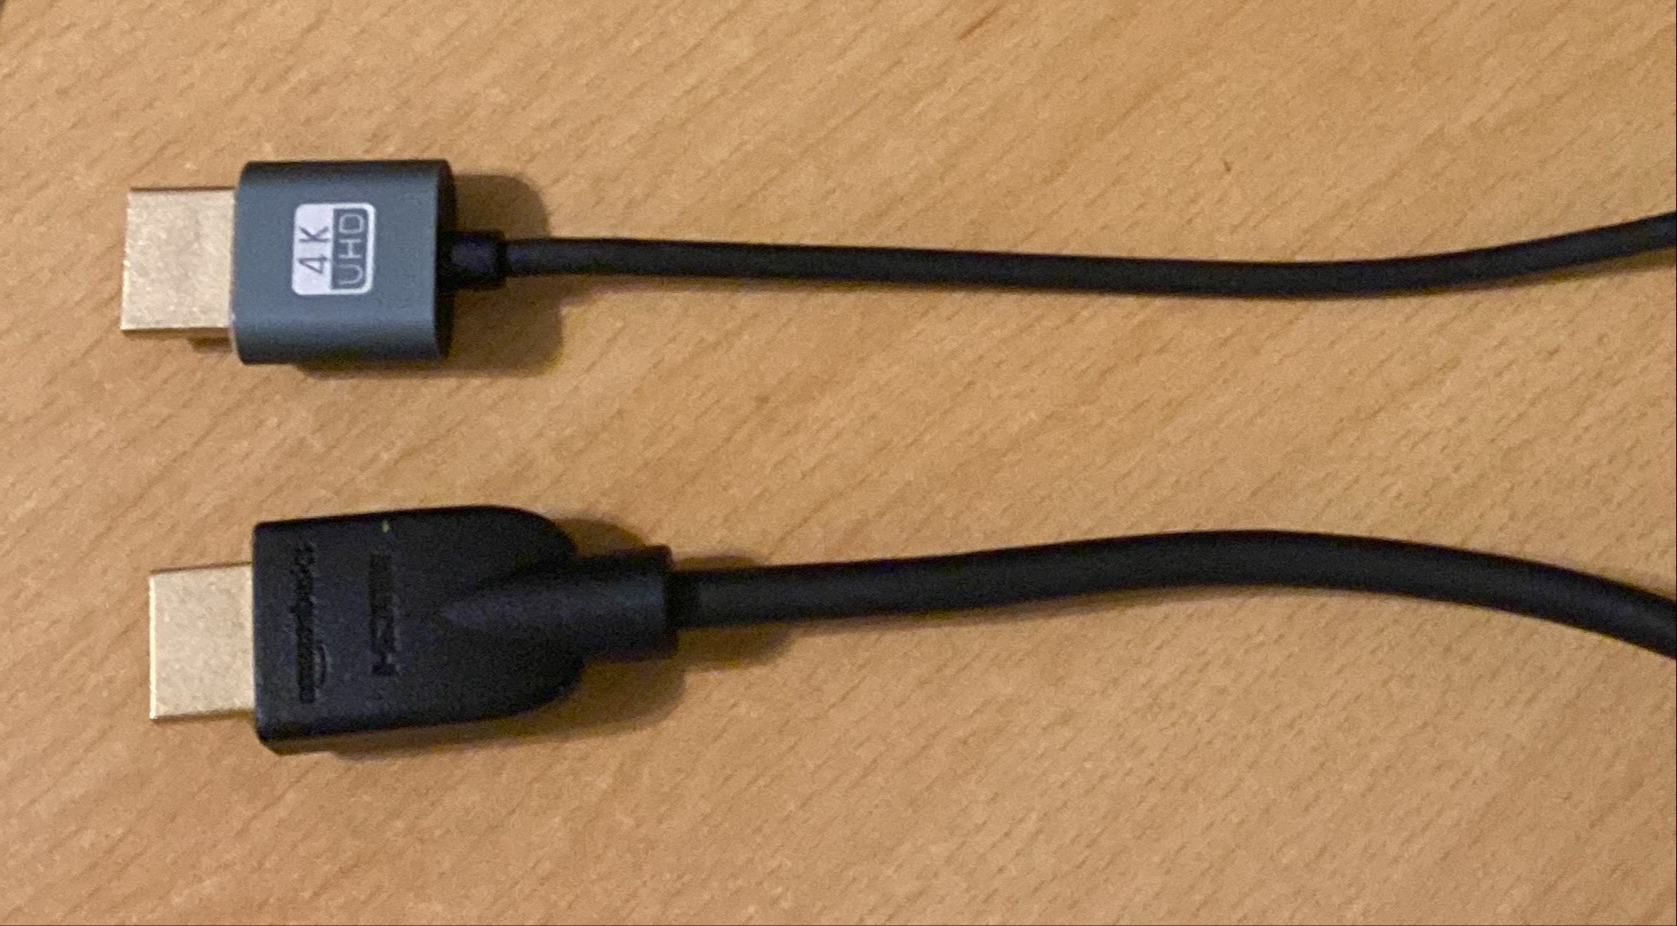
\includegraphics[width=0.7\linewidth]{images/bad-and-good-video-cables.jpg}
\end{figure}
    
    \subsection{No lights when powering on}
    If there are occasions when your MEGA65 display any lights when powering on, they relate to having certain Digital Video devices plugged in while the MEGA65 is off, that don't provide enough power for the keyboard's CPLD to be properly powered on, but enough to stop it properly resetting when the MEGA65 powers on. Removing the Digital Video cable and switching the machine off and on again fixes the issue.

\section{Vivado}
    \subsection{RAM requirements}
    \begin{tcolorbox}[colback=black,coltext=white]
    \begin{lstlisting}
INFO: [Synth 8-256] done synthesizing module 'ram32x1024' [/home/....]
INFO: [Synth 8-256] synthesizing module 'charrom' [/home/....]
    /opt/Xilinx/Vivado/2019.2/bin/loader: line 280: 2317 killed
    WARNING: [Vivado 12-8222] Failed run(s) : 'synth\_1'
        ERROR: Application Exception: failed to launch run 'impl\_1' due to failures in the following run(s):
        synth\_1
        These failed run(s) need to be reset prior to launching 'impl\_1' again.
    \end{lstlisting}
    \end{tcolorbox}
This error is due to Vivado crashing because the machine doesn't have enough RAM for Vivado to run.
Vivado requires at least 4GB to synthesise the MEGA65 target, but 8GB is better.

\section{mega65\_ftp}
    \subsection{Missing Library}
    \begin{tcolorbox}[colback=black,coltext=white]
\begin{lstlisting}
/usr/bin/ld: cannot find -lncurses
collect2: error: ld returned 1 exit status
Makefile:474: recipe for target 'bin/mega65_ftp' failed
make: *** [bin/mega65_ftp] Error 1\end{lstlisting}
    \end{tcolorbox}
This error occurs when the ncurses library is missing from the computer when building the mega65\_ftp program.
To rectify this issue you will need to ensure that you install this dependency.

    \begin{tcolorbox}[colback=black,coltext=white]
\begin{lstlisting}
sudo apt-get install libncurses5-dev libncursesw5-dev\end{lstlisting}
    \end{tcolorbox}

